\documentclass[journal,12pt,twocolumn]{IEEEtran}
\usepackage{cite}
\usepackage{amsmath,amssymb,amsfonts,amsthm}
\usepackage{algorithmic}
\usepackage{graphicx}
\usepackage{textcomp}
\usepackage{xcolor}
\usepackage{txfonts}
\usepackage{listings}
\usepackage{enumitem}
\usepackage{mathtools}
\usepackage{gensymb}
\usepackage{comment}
\usepackage[breaklinks=true]{hyperref}
\usepackage{tkz-euclide}
\usepackage{textgreek}
\usepackage{circuitikz}
\usepackage{pgfplots}
\usepackage[latin1]{inputenc}
\usepackage{color}
\usepackage{array}
\usepackage{longtable}
\usepackage{calc}
\usepackage{multirow}
\usepackage{hhline}
\usepackage{ifthen}
\usepackage{lscape}

\newtheorem{theorem}{Theorem}[section]
\newtheorem{problem}{Problem}
\newtheorem{proposition}{Proposition}[section]
\newtheorem{lemma}{Lemma}[section]
\newtheorem{corollary}[theorem]{Corollary}
\newtheorem{example}{Example}[section]
\newtheorem{definition}[problem]{Definition}
\newcommand{\BEQA}{\begin{eqnarray}}
\newcommand{\EEQA}{\end{eqnarray}}
\newcommand{\define}{\stackrel{\triangle}{=}}
\theoremstyle{remark}
\newtheorem{rem}{Remark}

\begin{document}
    \bibliographystyle{IEEEtran}
    \vspace{3cm}
    
    \title{GATE 23 EE Q38}
    \author{EE23BTECH11204 - Ashley Ann Benoy$^{*}$}% <-this % stops a space
    \maketitle
    \newpage
    \bigskip
    
    \bibliographystyle{IEEEtran}
    
    \textbf{Question: }
    Consider a lead compensator of the form
    \[ K(s) = \frac{1 + \frac{s}{a}}{1 + \frac{s}{\beta a}}, \quad \beta > 1, \quad a > 0 \]
    
    The frequency at which this compensator produces maximum phase lead is \(4 \, \text{rad/s}\). At this frequency, the gain amplification provided by the controller, assuming an asymptotic Bode-magnitude plot of \(K(s)\), is \(6 \, \text{dB}\). The values of \(a\) and \(\beta\), respectively, are
    
    \[
    \text{(A)} \, 1, 16 \quad
    \text{(B)} \, 2, 4 \quad
    \text{(C)} \, 3, 5 \quad
    \text{(D)} \, 2.66, 2.25
    \]
    
    \textbf{Solution:}
     \begin{table}[h]
        \centering
        \begin{tabular}{|c|c|}
            \hline
            \textbf{Parameter} & \textbf{Value} \\
            \hline
            Transfer Function & \( K(s) = \frac{1 + \frac{s}{a}}{1 + \frac{s}{\beta a}} \) \\
            \hline
            Maximum Phase Lead Frequency & \( \omega_m = 4 \, \text{rad/s} \) \\
            \hline
            Gain Amplification at \( \omega_m \) & \( 20\log_{10}|K(j\omega_m)| = 6 \, \text{dB} \) \\
            \hline
            Conditions & \( \beta > 1, \, a > 0 \) \\
            \hline
        \end{tabular}
        \caption{Given Parameters}
        \label{tab:given-parameters}
    \end{table}

   
    
    \[ K(s) = \frac{1 + \frac{s}{a}}{1 + \frac{s}{a\beta}} \]
    
    \begin{align}
    K(s) &= \frac{s + a}{a} \cdot \frac{a\beta}{s + a\beta} \\
    &= \beta \frac{s + a}{s + a\beta}
    \end{align}
    
    1. The max phase lead is: \(\omega_m = \sqrt{a \cdot a \cdot \beta}\)\\

    2. If \(G(s) = \frac{k(s+a)}{s(s+a\beta)}\) has to act as a lead compensator, then \(a\beta\) must be greater than \(a\), i.e., \(a\beta > a \).\\
    
  
    
    Using the above properties we have:
    
    \begin{align}
    \omega_m &= \sqrt{ a \cdot a \beta}=4 \\
    \beta &> 1
    \end{align}
    
    \begin{align}
    K(j\omega) &= \frac{1 + \frac{j\omega}{a}}{1 + \frac{j\omega}{a\beta}} 
    &= \beta \frac{j\omega + a}{j\omega + a\beta}
    \end{align}
    
    \begin{align}
    |K(j\omega)| =\frac{\beta \sqrt{\omega^2 + a^2}}{\sqrt{\omega^2 + (a\beta)^2}}
    \end{align}
    
    Using Gain Amplification:
    \begin{align}
     20\log_{10}|K(j\omega_m)| = 6
     \end{align}
     \begin{align}
     |K(j\omega_m)| \approx  2
     \end{align}
     
    \begin{align}
    |K(j\omega_m)| =\frac{\beta \sqrt{(\omega_m)^2 + a^2}}{\sqrt{(\omega_m)^2 + (a\beta)^2}}=2
    \end{align}
    
    \begin{align}
    \frac{\beta \sqrt{16 + a^2}}{\sqrt{16 + (a\beta)^2}}=2
    \end{align}
    
    Solving the above equation, we get \(a \approx 2\) and \(\beta = 4\). Therefore, the correct answer is \textbf{(B) 2, 4}.
    
    The Bode plots for the same are as follows:
    \begin{figure}[h!]
  \centering
  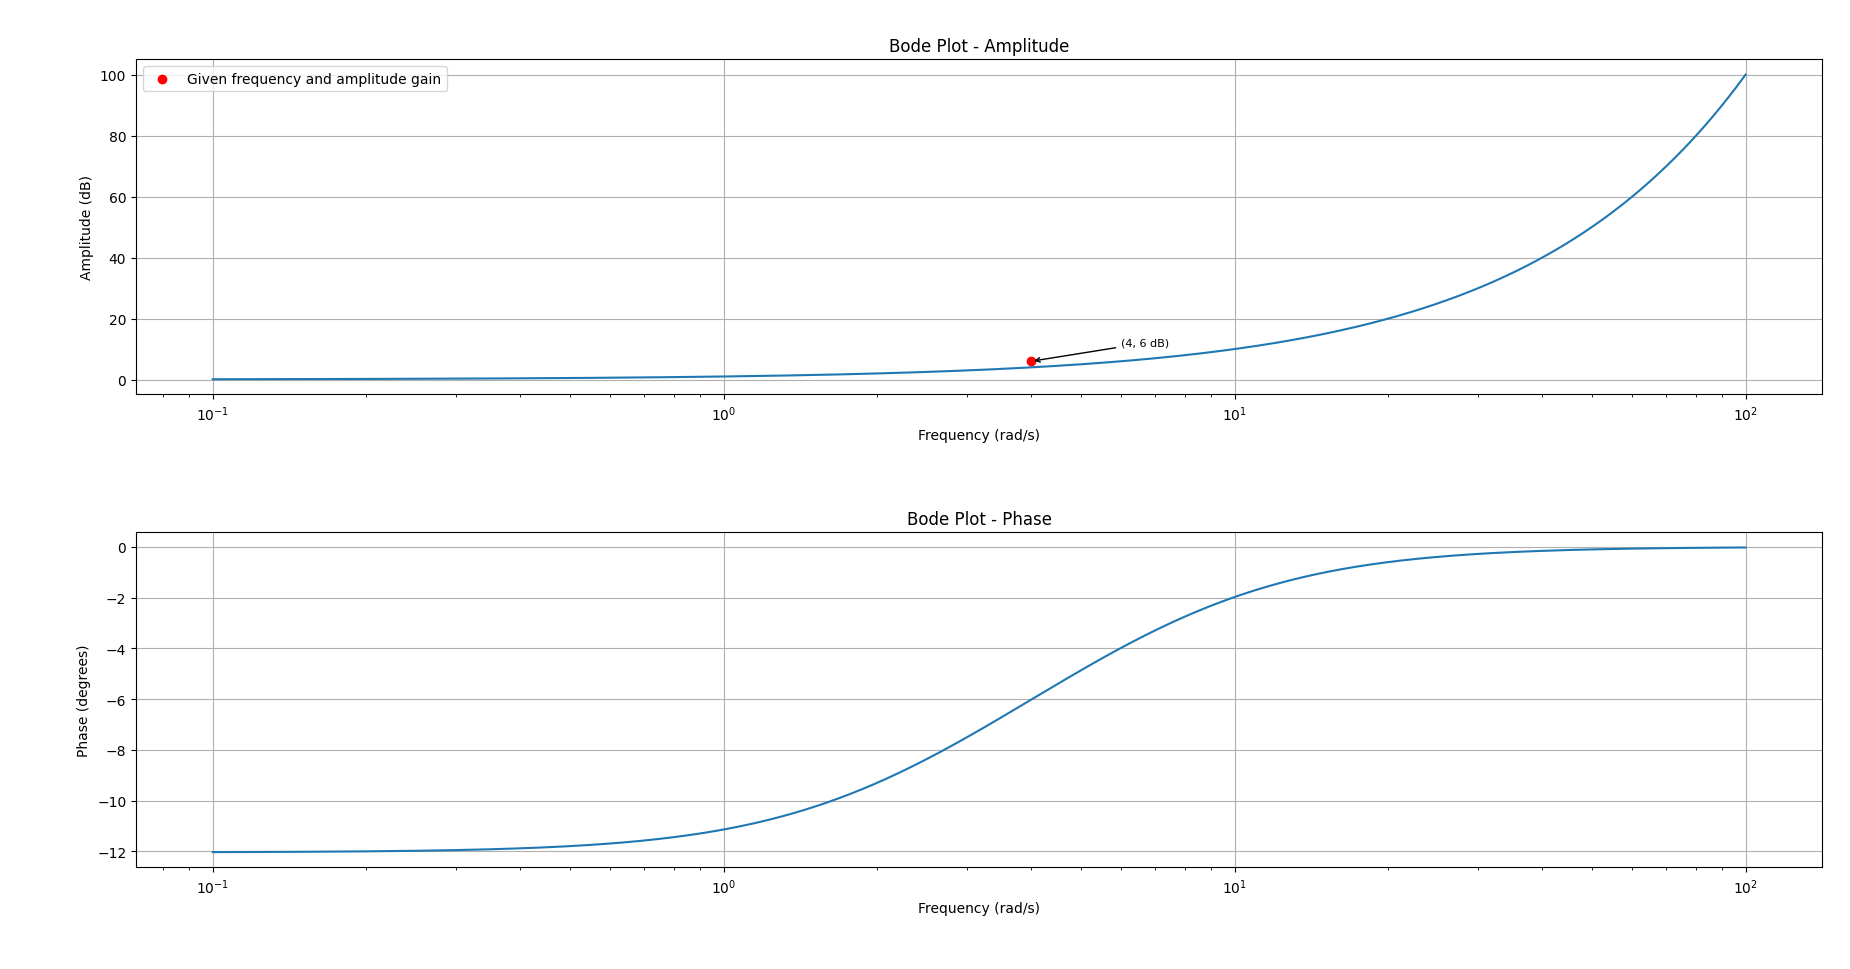
\includegraphics[width=\columnwidth]{figs/bode.png}
  \label{fig:bode_Plot}
\end{figure}
\end{document}
